\ifx\pdfminorversion\undefined\else\pdfminorversion=4\fi
\documentclass[aspectratio=169,t]{beamer}
%\documentclass[aspectratio=169,t,handout]{beamer}

% English version FAU Logo
\usepackage[english]{babel}
% German version FAU Logo
%\usepackage[ngerman]{babel}

\usepackage[utf8]{inputenc}
\usepackage[T1]{fontenc}
\usepackage{amsmath,amssymb}
\usepackage{graphicx}
\usepackage{listings}
\usepackage{url}
\usepackage{enumitem}
\usepackage{hyperref}
\usepackage{fontawesome}
\usepackage{graphicx}
\usepackage{booktabs}
\usepackage{calc}
\usepackage{ifthen}
\usepackage{xcolor}
\usepackage{tikz}
\usepackage{tikz}
\usepackage{tikz-cd}
\usepackage{pgfplots,pgfplotstable,pgf-pie}
\usepackage{filecontents}
\newcommand{\plots}{0.611201}
\newcommand{\plotm}{2.19882}
\pgfplotsset{height=4cm,width=8cm,compat=1.17}
\pgfmathdeclarefunction{gauss}{2}{%
  \pgfmathparse{1/(#2*sqrt(2*pi))*exp(-((x-#1)^2)/(2*#2^2))}%
}

\tikzset{
    vertex/.style = {
        circle,
        fill            = black,
        outer sep = 2pt,
        inner sep = 1pt,
    }
}
\usetikzlibrary{matrix,mindmap}
\usetikzlibrary{arrows,decorations.pathmorphing,backgrounds,fit,positioning,shapes.symbols,chains,intersections,snakes,positioning}
\tikzset{level 1/.append style={sibling angle=50,level distance = 165mm}}
\tikzset{level 2/.append style={sibling angle=20,level distance = 45mm}}
\tikzset{every node/.append style={scale=1}}
% read in data file
\pgfplotstableread{data/iris.dat}\iris
% get number of data points
\pgfplotstablegetrowsof{\iris}
\pgfmathsetmacro\NumRows{\pgfplotsretval-1}
\definecolor{airforceblue}{rgb}{0.36, 0.54, 0.66}
\usepgfplotslibrary{groupplots}
\pgfplotsset{compat=1.14}
\newcommand{\tikzmark}[1]{\tikz[remember picture] \node[coordinate] (#1) {#1};}
% Options:
%  - inst:      Institute
%                 med:      MedFak FAU theme
%                 nat:      NatFak FAU theme
%                 phil:     PhilFak FAU theme
%                 rw:       RWFak FAU theme
%                 rw-jura:  RWFak FB Jura FAU theme
%                 rw-wiso:  RWFak FB WISO FAU theme
%                 tf:       TechFak FAU theme
%  - image:     Cover image on title page
%  - plain:     Plain title page
%  - longtitle: Title page layout for long title
\usetheme[%
  image,%
  longtitle,%
  tf
]{fau}

% Enable semi-transparent animation preview
\setbeamercovered{transparent}


\lstset{%
  language=Python,
  tabsize=2,
  basicstyle=\tt,
  keywordstyle=\color{blue},
  commentstyle=\color{green!50!black},
  stringstyle=\color{red},
  numbers=left,
  numbersep=0.5em,
  xleftmargin=1em,
  numberstyle=\tt
}


% Title, authors, and date
\title[KDD]{Chapter IV: Preprocessing}
\subtitle{Knowledge Discovery in Databases}
\author[L.~Melodia]{Luciano Melodia M.A.}
% English version
\institute[Department]{Evolutionary Data Management, Friedrich-Alexander University Erlangen-Nürnberg}
% German version
%\institute[Lehrstuhl]{Lehrstuhl, Friedrich-Alexander-Universit\"at Erlangen-N\"urnberg}
\date{Summer semester 2021}
% Set additional logo (overwrites FAU seal)
%\logo{\includegraphics[width=.15\textwidth]{themefau/art/xxx/xxx.pdf}}
\begin{document}
  % Title
  \maketitle

  { 
    \setbeamertemplate{footline}{}
    \begin{frame}{Chapter IV: Preprocessing}
    This is our agenda for this lecture:
        \begin{itemize}
            \item \textbf{Data preprocessing: an overview.}
            \begin{itemize}
              \item Data quality.
              \item Major tasks in data preprocessing.
            \end{itemize}
            \item Data cleaning.
            \item Data integration.
            \item Data reduction.
            \item Data transformation and data discretization.
            \item Summary.
        \end{itemize}
    \end{frame}
  }

  { 
    \setbeamertemplate{footline}{}
    \begin{frame}{Data quality: why preprocess the data?}
    This is our agenda for this lecture:
        \begin{itemize}
            \item \textbf{Measures for {\color{airforceblue}data quality}: A multidimensional view:}
            \begin{itemize}
              \item \textbf{Accuracy:} correct or wrong, accurate or not.
              \item \textbf{Completeness:} not recorded, unavailable.
              \item \textbf{Consistency:} some modified but some not, dangling refs, etc.
              \item \textbf{Timeliness:} timely updated?
              \item \textbf{Believability:} how trustworthy is it, that the data is correct?
              \item \textbf{Interpretability:} how easily can the data be understood?
              \item And even many more!
            \end{itemize}
        \end{itemize}
    \end{frame}
  }

  { 
    \setbeamertemplate{footline}{}
    \begin{frame}{Major tasks in data preprocessing}
      \begin{itemize}
        \item \textbf{Data cleaning:}
        \begin{itemize}
          \item Fill in missing values.
          \item Smooth noisy data.
          \item Identify or remove outliers.
          \item Resolve inconsistencies.
        \end{itemize}
        \item \textbf{Data integration:}
        \begin{itemize}
          \item Integration of multiple databases.
          \item Data cubes or files.
        \end{itemize}
        \item \textbf{Data reduction:}
        \begin{itemize}
          \item Dimensionality reduction.
          \item Numerosity reduction.
          \item Data compression.
        \end{itemize}
        \item \textbf{Data transformation and data discretization:}
        \begin{itemize}
          \item Normalization.
          \item Concept-hierarchy generation.
        \end{itemize}
      \end{itemize}
    \end{frame}
  }

  { 
    \setbeamertemplate{footline}{}
    \begin{frame}{Chapter IV: Preprocessing}
        \begin{itemize}
            \item Data preprocessing: an overview.
            \begin{itemize}
              \item Data quality.
              \item Major tasks in data preprocessing.
            \end{itemize}
            \item \textbf{Data cleaning.}
            \item Data integration.
            \item Data reduction.
            \item Data transformation and data discretization.
            \item Summary.
        \end{itemize}
    \end{frame}
  }

  { 
    \setbeamertemplate{footline}{}
    \begin{frame}{Data cleaning}
      \textbf{Data in the real world is {\color{airforceblue}dirty}. Lots of potentially incorrect data:}
      \begin{itemize}
        \item E.g. instrument faukty, human or computer error, transmission error.
        \item \textbf{\color{airforceblue}Incomplete:} lacking attributes, lacking certain attributes of interest or containing aggregate data.
        \begin{itemize}
          \item E.g. occupation = "" (missing data).
        \end{itemize}
        \item \textbf{\color{airforceblue}Noisy:} containing noise, errors or outliers.
        \begin{itemize}
          \item Stochastic deviation, imprecision.
          \item E.g. measurements.
        \end{itemize}
        \item \textbf{\color{airforceblue}Inconsistencies:} containing discrepancies in codes or names.
        \begin{itemize}
          \item E.g. age = "42", birthday = "03/07/2010".
          \item Was rating "1,2,3" and now it is "A,B,C".
          \item Discrepancy between duplicate records (e.g. address old and new).
        \end{itemize}
        \item \textbf{\color{airforceblue}Intentional} (only default value, e.g. disguised missing data):
        \begin{itemize}
          \item Jan. 1 as everyone's birthday?
        \end{itemize}
      \end{itemize}
    \end{frame}
  }

  { 
    \setbeamertemplate{footline}{}
    \begin{frame}{Incomplete (missing) data}
    \begin{itemize}
      \item \textbf{Data is not always available.}
      \begin{itemize}
        \item E.g. many tuples have no recorded value for several attributes.
        \item Examples are customer income in sales data.
      \end{itemize}
      \item \textbf{Missing data may be due to:}
      \begin{itemize}
        \item Equipment malfunction.
        \item Inconsistency with other recorded data and thus deleted.
        \item Data not entered due to misunderstanding.
        \item Certain data may not be considered important at the time of entry.
        \item Not registered history or changes of the data.
      \end{itemize}
      \item \textbf{Missing data may need to be inferred.}
    \end{itemize}
    \end{frame}
  }

  { 
    \setbeamertemplate{footline}{}
    \begin{frame}{How to handle missing data?}
    \begin{itemize}
      \item \textbf{Ignore the tuple:}
      \begin{itemize}
        \item Usually done when class label is missing (when doing classification).
        \item Not effective when the percentage of missing values per attribute varies considerably.
      \end{itemize}
      \item \textbf{Fill in the missing value manually.}
      \begin{itemize}
        \item Tedious or infeasible.
      \end{itemize}
      \item \textbf{Fill in automatically with:}
      \begin{itemize}
        \item A global constant, e.g. "unkown", maybe a new class.
        \item The attribute mean.
        \item The attribute mean for all samples belonging to the same class.
        \item \textbf{\color{airforceblue} The most probable value:} Inference-based such as Bayesian formula or decision tree.
      \end{itemize}
    \end{itemize}
    \end{frame}
  }

  { 
    \setbeamertemplate{footline}{}
    \begin{frame}{Noisy data?}
    \begin{itemize}
      \item \textbf{\color{airforceblue}Noise:}
      \begin{itemize}
        \item Random error or variance in a measured variable.
        \item Stored value a little bit off the real value, up or down.
        \item Leads to (slightly) incorrect attribute values.
      \end{itemize}
      \item \textbf{May be due to:}
      \begin{itemize}
        \item Faulty or imprecise data-collection instruments.
        \item Data-entry problems.
        \item Data-transmission problems.
        \item Technology limitation.
        \item Inconsistency in naming conventions.
      \end{itemize}
    \end{itemize}
    \end{frame}
  }

  { 
    \setbeamertemplate{footline}{}
    \begin{frame}{How to handle noisy data?}
    \begin{itemize}
        \item \textbf{Beginning:}
        \begin{itemize}
          \item First sort data and partition into (equal-frequency) bins.
          \item Then smooth by bin mean, by bin median or by bin boundaries.
        \end{itemize}
        \item \textbf{Regression:}
        \begin{itemize}
          \item Smooth by fitting the data to regression functions.
        \end{itemize}
        \item \textbf{Clustering:}
        \begin{itemize}
          \item Detect and remove outliers.
        \end{itemize}
        \item \textbf{Combined computer and human inspection:}
        \begin{itemize}
          \item Detect suspicious values and check by human.
          \item E.g. deal with possible outliers.
        \end{itemize}
    \end{itemize}
    \end{frame}
  }

 { 
    \setbeamertemplate{footline}{}
    \begin{frame}{Data cleaning as a process}
    \begin{itemize}
      \item \textbf{Data-discrepancy detection:}
      \begin{itemize}
        \item Use \textbf{\color{airforceblue}metadata} (e.g. domain, range, dependency, distribution).
        \item Check field overloading.
        \item Check uniqueness rule, consecutive rule and null rule.
        \item Use commercial tools:
        \begin{itemize}
          \item \textbf{\color{airforceblue}Data scrubbing:} use simple domain knowledge (e.g. postal code, spell-check) to detect errors and make corrections.
          \item \textbf{\color{airforceblue}Data auditing:} by analyzing data to discover rules and relationsships to detect violators (e.g. correlation and clustering to find outliers).
        \end{itemize}
        \item \textbf{Data migration and integration:}
        \begin{itemize}
          \item Data-migration tools: allow transformations to be specified.
          \item ETL (Extraction/Transformation/Loading) tools: allow users to specify transformations through a graphical user interface.
        \end{itemize}
        \item \textbf{Integration of the two processes.}
        \begin{itemize}
          \item Iterative and interactive (e.g. the Potter's Wheel tool).
        \end{itemize}
      \end{itemize}
    \end{itemize}
    \end{frame}
  }

  { 
    \setbeamertemplate{footline}{}
    \begin{frame}{Chapter IV: Preprocessing}
        \begin{itemize}
            \item Data preprocessing: an overview.
            \begin{itemize}
              \item Data quality.
              \item Major tasks in data preprocessing.
            \end{itemize}
            \item Data cleaning.
            \item \textbf{Data integration.}
            \item Data reduction.
            \item Data transformation and data discretization.
            \item Summary.
        \end{itemize}
    \end{frame}
  }

  { 
    \setbeamertemplate{footline}{}
    \begin{frame}{Data integration}
    \begin{itemize}
       \item \textbf{Data integration:}
       \begin{itemize}
        \item Combine data from multiple sources into a coherent store.
       \end{itemize}
       \item \textbf{Schema integration:}
       \begin{itemize}
        \item E.g. \texttt{A.cust-id} $\equiv$ \texttt{B.cust-\#}.
        \item Integrate metadata from different sources.
       \end{itemize}
       \item \textbf{Entity-identification problem:}
       \begin{itemize}
        \item Identify the same real-world entities from multiple data sources.
        \item E.g. Bill Clinton = William Clinton.
       \end{itemize}
       \item \textbf{Detecting and resolving {\color{airforceblue}data-value conflicts}:}
       \begin{itemize}
        \item For the same real world entity, attribute values from different sources are different.
        \item Possible reasons:
        \begin{itemize}
          \item Different representations (coding).
          \item Different scales, e.g. metric vs. British units.
        \end{itemize}
       \end{itemize}
    \end{itemize}
    \end{frame}
  }

  { 
    \setbeamertemplate{footline}{}
    \begin{frame}{Handling redundancy in data integration}
    \begin{itemize}
      \item \textbf{Redundant data often occur when integrating multiple databases.}
      \begin{itemize}
        \item \textbf{Object (entity) identification:} \\
              The same attribute or object may have different names in different databases.
        \item \textbf{Derivable data:}\\
              One attribute may be a "derived" attribute in another table. E.g. annual revenue.
      \end{itemize}
      \item \textbf{Redundant attributes:}
      \begin{itemize}
        \item Can be detected by \textbf{\color{airforceblue}correlation analysis} and \textbf{\color{airforceblue}covariance analysis}.
      \end{itemize}
      \item \textbf{Careful integration of the data from multiple sources:}
      \begin{itemize}
        \item Helps to reduce\/avoid redundancies and inconsistencies and improve mining speed and quality.
      \end{itemize}
    \end{itemize}
    \end{frame}
  }

  { 
    \setbeamertemplate{footline}{}
    \begin{frame}{Correlation analysis for nominal data (I)}
      \begin{itemize}
        \item \textbf{Two attributes:}
        \begin{itemize}
          \item $A$ has $n$ distinct values: $A := \{a_1, a_2, \ldots, a_n\}$.
          \item $B$ has $m$ distinct values: $B := \{b_1, b_2, \ldots, b_m\}$.
        \end{itemize}
        \item \textbf{\color{airforceblue}Contingency table:}
        \begin{itemize}
          \item Columns: the $n$ values of $A$.
          \item Rows: the $m$ values of $B$.
          \item Cells: counts of records with \\
          $A' = \{ a_i \in A \; : \; a_i = a_k \; \text{for} \; a_k \in A\}$ and \\
          $B' = \{ b_j \in B \; : \; b_j = b_l \; \text{for} \; b_l \in B\}$.
        \end{itemize}
        \item \textbf{Expected count in cell $(i,j)$:}
        \begin{align}
          e_{ij} = \frac{\#A' \cdot \#B'}{\#A + \#B},
        \end{align}
        \item where $\#A + \#B$ is the total number of records.
      \end{itemize}
    \end{frame}
  }

  { 
    \setbeamertemplate{footline}{}
    \begin{frame}{Correlation analysis for nominal data (II)}
      \begin{itemize}
        \item \textbf{\color{airforceblue}$\chi^2$-test:}
        \begin{align}
          \chi^2 = \sum_{i=1}^{N} \frac{(x_i-\hat{x}_i)^2}{\hat{x}_i}.
        \end{align}
        \item Summing over all cells of the contingency table.
        \item No correlation (i.e. independence of attributes) yields $\chi^2$ value of zero.
        \item The larger the $\chi^2$ value, the more likely the variables are related.
        \item The cells that contribute the most to the $\chi^2$ value
are those whose actual count is very different from the expected count.
      \end{itemize}
      \begin{itemize}
        \item \textbf{Correlation does not imply causality!}
        \item E.g. $\#$ of hospitals and $\#$ of car-thefts in a city are correlated.
        \item Both are causally linked to the third variable: population.
      \end{itemize}
    \end{frame}
  }

  { 
    \setbeamertemplate{footline}{}
    \begin{frame}{$\xi^2$ calculation: an example}
    \centering
    \begin{tabular}{l|c|c|c|}
    & Play chess & Not play chess & Sum (row)\\\hline
    Like Science fiction & $250 (90)$ & $200 (360)$ & $450$ \\\hline
    Not like science fiction & $50 (210$ & $1000 (840)$ & $1050$\\\hline
    Sum (column) & $300$ & $1200$ & $1500$\\\hline
    \end{tabular}
    \begin{itemize}
      \item Numbers in parenthesis are expected counts calculated based on the data distribution in the two categories.
      \item $\chi^2$ calculation:
      \begin{align}
      \chi^2 = \frac{(250-90)^2}{90} + \frac{(50-210)^2}{210} + \frac{(200-360)^2}{360} + \frac{(1000-840)^2}{840} = 507.93.
      \end{align}
      \item It shows that "like science fiction" and "play chess" are correlated in the group.
    \end{itemize}
    \end{frame}
  }

  { 
    \setbeamertemplate{footline}{}
    \begin{frame}{Correlation analysis of numerical data}
    \begin{itemize}
      \item \textbf{\color{airforceblue}Correlation coefficient:}
      \begin{itemize}
        \item Also called Pearson's product-moment coefficient
        \begin{align}
          r_{A,B} = \frac{\sum_{i=1}^{N + M} (a_i-\mu_A)(b_i-\mu_B)}{(N+M-1)\sigma_A\sigma_B} = \frac{\sum_{i=1}^{N+M}(a_ib_i)-(N+M)\mu_A\mu_B}{(N+M-1) \sigma_A\sigma_B}.
        \end{align}
        where $N = \# A$, $M = \# B$, $\mu_A$ and $\mu_B$ are the means of $A$ and $B$, respectively. $\sigma_A$ and $\sigma_B$ denote the corresponding standard deviations.
      \end{itemize}
      \item If $r_{A,B} > 0$, $A$ and $B$ are positively correlated ($A$'s values increase with $B$'s). \\
      The higher, the stronger the correlation.
      \item $r_{A,B} = 0$: independent.
      \item $r_{A,B} < 0$: negatively correlated.
    \end{itemize}
    \end{frame}
  }

  { 
    \setbeamertemplate{footline}{}
    \begin{frame}{Visually evaluating correlation}
    \begin{figure}[H]
        \centering
        \begin{minipage}{0.32\textwidth}
            \centering
            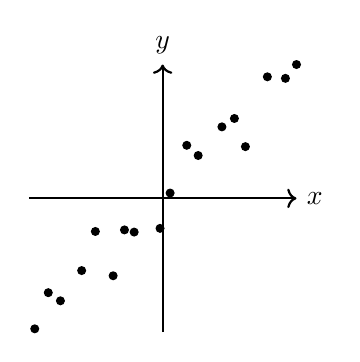
\begin{tikzpicture}
            \draw[->, thick] (-1.7,0)--(1.7,0) node[right]{$x$};
            \draw[->, thick] (0,-1.7)--(0,1.7) node[above]{$y$};
            \foreach \x in {-1.7,-1.5,...,1.7}{
                    \pgfmathsetmacro\xcoord{\x+rand/10}
                    \pgfmathsetmacro\ycoord{\x+rand/2}
                    \pgfmathsetmacro\xcoord{\xcoord < -1.7 ? -1.7 : \xcoord}
                    \pgfmathsetmacro\xcoord{\xcoord > 1.7 ? 1.7 : \xcoord}
                    \pgfmathsetmacro\ycoord{\ycoord < -1.7 ? -1.7 : \ycoord}
                    \pgfmathsetmacro\ycoord{\ycoord > 1.7 ? 1.7 : \ycoord}
                    \node[circle,draw,fill=black,scale=0.3] at (\xcoord,\ycoord) {};
                }
            \end{tikzpicture}
            \caption{a) Positive correlation.}
        \end{minipage}\hfill
        \begin{minipage}{0.32\textwidth}
            \centering
            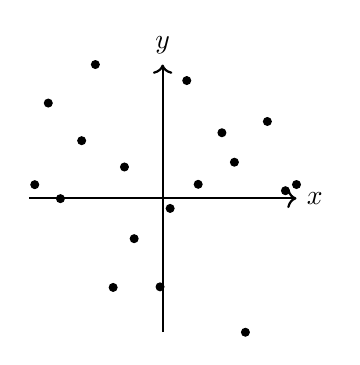
\begin{tikzpicture}
            \draw[->, thick] (-1.7,0)--(1.7,0) node[right]{$x$};
            \draw[->, thick] (0,-1.7)--(0,1.7) node[above]{$y$};
            \foreach \x in {-1.7,-1.5,...,1.7}{
                    \pgfmathsetmacro\xcoord{\x+rand/10}
                    \pgfmathsetmacro\ycoord{rand*2}
                    \pgfmathsetmacro\xcoord{\xcoord < -1.7 ? -1.7 : \xcoord}
                    \pgfmathsetmacro\xcoord{\xcoord > 1.7 ? 1.7 : \xcoord}
                    \pgfmathsetmacro\ycoord{\ycoord < -1.7 ? -1.7 : \ycoord}
                    \pgfmathsetmacro\ycoord{\ycoord > 1.7 ? 1.7 : \ycoord}
                    \node[circle,draw,fill=black,scale=0.3] at (\xcoord,\ycoord) {};
                }
            \end{tikzpicture}
            \caption{b) Uncorrelated/no correlation.}
        \end{minipage}\hfill
        \begin{minipage}{0.32\textwidth}
            \centering
            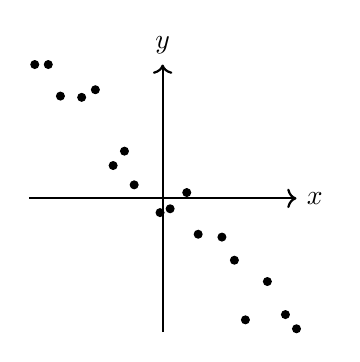
\begin{tikzpicture}
            \draw[->, thick] (-1.7,0)--(1.7,0) node[right]{$x$};
            \draw[->, thick] (0,-1.7)--(0,1.7) node[above]{$y$};
            \foreach \x in {-1.7,-1.5,...,1.7}{
                    \pgfmathsetmacro\xcoord{\x+rand/10}
                    \pgfmathsetmacro\ycoord{-\x+rand/2}
                    \pgfmathsetmacro\xcoord{\xcoord < -1.7 ? -1.7 : \xcoord}
                    \pgfmathsetmacro\xcoord{\xcoord > 1.7 ? 1.7 : \xcoord}
                    \pgfmathsetmacro\ycoord{\ycoord < -1.7 ? -1.7 : \ycoord}
                    \pgfmathsetmacro\ycoord{\ycoord > 1.7 ? 1.7 : \ycoord}
                    \node[circle,draw,fill=black,scale=0.3] at (\xcoord,\ycoord) {};
                }
            \end{tikzpicture}
            \caption{c) Negative correlation.}
        \end{minipage}\hfill
    \end{figure} 
    \end{frame}
  }

  { 
    \setbeamertemplate{footline}{}
    \begin{frame}{Covariance of numerical data (I)}
    \begin{itemize}
      \item \textbf{\color{airforceblue}Covariance} \textbf{is similar to correlation:}\\
            \begin{align}
              \text{Cov}(A,B) = \frac{\sum_{i=1}^{n}(a_i-\overline{A})(b_i-\overline{B})}{n}
            \end{align}
      \item \textbf{Pearson's correlation coefficient:}\\
            \begin{align}
              r = \frac{n \sum_{i=1}^{n}a_ib_i - \sum_{i=1}^{n}a_i \sum_{i=1}^{n}b_i}{\sqrt{\left(n \left(\sum_{i=1}^{n} a^2\right) - \left(\sum_{i=1}^{n} a_i\right)^2\right) \left(n \left(\sum_{i=1}^{n}b^2\right) - \left(\sum_{i=1}^{n}b_i\right)^2\right)}},
            \end{align}
            where $n$ is the number of tuples.
    \end{itemize}
    \end{frame}
  }


  { 
    \setbeamertemplate{footline}{}
    \begin{frame}{Covariance of numerical data (II)}
    \begin{itemize}
      \item \textbf{Positive covariance:}\\
            If $\text{Cov}(A,B) > 0$, then $A$ and $B$ tend to be either both larger or both smaller than their expected values.
      \item \textbf{Negative covariance:}\\
            If $\text{Cov}(A,B) < 0$, then if $A$ is larger than its expected value, $B$ is likely to be smaller than its expected value and vice versa.
      \item \textbf{Independence:}
      \begin{itemize}
        \item $\text{Cov}(A,B) = 0$.
        \item \textbf{\color{airforceblue}But the converse is not true:} Some pairs of random variables may have a covariance of $0$ but are not independent. Only under some additional assumptions (e.g., the data follow multivariate normal distributions) does a covariance of $0$ imply independence.
      \end{itemize}
    \end{itemize}
    \end{frame}
  }

  { 
    \setbeamertemplate{footline}{}
    \begin{frame}{Covariance: an example (I)}
    \begin{itemize}
      \item \textbf{Can be simplified in computation as:}
            \begin{align}
              \text{Cov}(A,B) &= E(A - E(A))(B-E(B))\\
                              &= E(AB-AE(B)-E(A)B+E(A)E(B))\\
                              &= E(AB)-E(A)E(B)-E(A)E(B)+E(A)E(B)\\
                              &= E(AB)-E(A)E(B).
            \end{align}
    \end{itemize}
    \end{frame}
  }


  { 
    \setbeamertemplate{footline}{}
    \begin{frame}{Covariance: an example (II)}
    \begin{itemize}
      \item Suppose two stocks $A$ and $B$ have the following values within some time:\\
      $(2,5), (3,8), (5,10), (4,11), (6,14).$
      \item If the stocks are affected by the same industry trends, will their prices rise or fall together?
      \begin{align}
        E(A) &= \frac{2+3+5+4+6}{5} = \frac{20}{5} = 4.\\
        E(B) &= \frac{5+8+10+11+14}{5} = \frac{48}{5} = 9.6.\\
        \text{Cov}(A,B) &= \frac{2\cdot5 + 3\cdot 8 + 5 \cdot 10 + 4 \cdot 11 + 6 \cdot 14}{5} - 4\cdot 9.6 = 4.
      \end{align}
      \item Thus, $A$ and $B$ rise together since $\text{Cov}(A,B) > 0$.
    \end{itemize}
    \end{frame}
  }

  { 
    \setbeamertemplate{footline}{}
    \begin{frame}{Chapter IV: Preprocessing}
        \begin{itemize}
            \item Data preprocessing: an overview.
            \begin{itemize}
              \item Data quality.
              \item Major tasks in data preprocessing.
            \end{itemize}
            \item Data cleaning.
            \item Data integration.
            \item \textbf{Data reduction.}
            \item Data transformation and data discretization.
            \item Summary.
        \end{itemize}
    \end{frame}
  }

  { 
    \setbeamertemplate{footline}{}
    \begin{frame}{Data reduction I: dimensionality reduction}
        \begin{itemize}
            \item \textbf{Curse of dimensionality:}
            \begin{itemize}
              \item When dimensionality increases data becomes increasingly sparse.
              \item Density and distance between points, which are critical to clustering and outlier analysis become less meaningful.
              \item The possible combinations of subspaces will grow exponentially.
            \end{itemize}
            \item \textbf{Dimensionality reduction:}
            \begin{itemize}
              \item Avoid the curse of dimensionality.
              \item Help eliminate irrelevant features and reduce noise.
              \item Reduce time and space required in data mining.
              \item Allow easier visualization.
            \end{itemize}
            \item \textbf{Dimensionality-reduction techniques:}
            \begin{itemize}
              \item Wavelet transforms.
              \item Principal component analysis.
              \item Supervised and nonlinear techniques (e.g. feature selection).
            \end{itemize}
        \end{itemize}
    \end{frame}
  }

  { 
    \setbeamertemplate{footline}{}
    \begin{frame}{Data reduction strategies}
        \begin{itemize}
            \item Obtain a reduced representation of the data set that is much smaller in volume but yet produces the same (or almost the same)  results.
            \item \textbf{Why data reduction?}\\
            \begin{itemize}
              \item A database/data warehouse may store terabytes of data.
              \item Complex data analysis may take a very long time to run on the complete data set.
            \end{itemize}
            \item \textbf{Data reduction strategies:}
            \begin{itemize}
              \item Dimensionality reduction, i.e. remove unimportant attributes.
              \begin{itemize}
                \item Wavelet transforms.
                \item Principal component analysis.
                \item Attribute subset selection or attribute creation.
              \end{itemize}
              \item Numerosity reduction:
              \begin{itemize}
                \item Regression and log-linear models.
                \item Histograms, clustering and sampling.
                \item Data cube aggregation.
              \end{itemize}
              \item Data compression.
            \end{itemize}
        \end{itemize}
    \end{frame}
  }

  { 
    \setbeamertemplate{footline}{}
    \begin{frame}{Mapping data to a new space}
    \begin{itemize}
      \item \textbf{Fourier transform}.
      \item \textbf{Wavelet transform.}

    \begin{figure}
      \centering
      \begin{minipage}[b]{0.30\textwidth}
        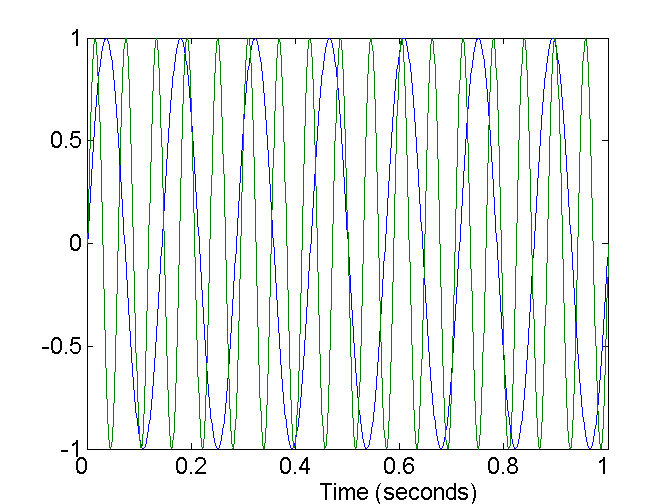
\includegraphics[width=5cm]{img/twosinewaves.png}
        \caption{Two sine waves.}
      \end{minipage}\hfill
      \begin{minipage}[b]{0.30\textwidth}
        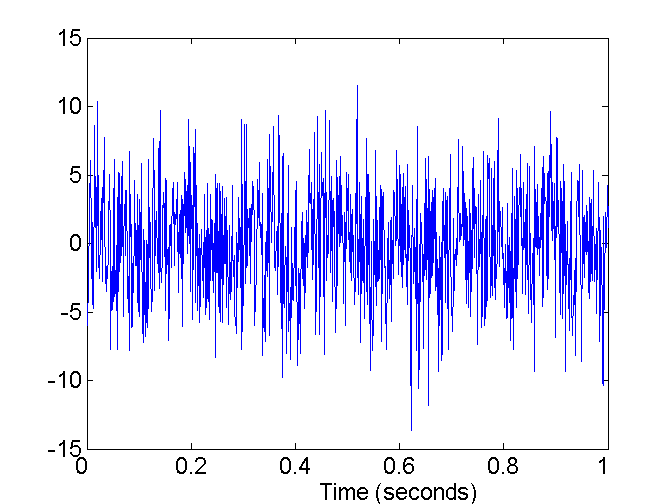
\includegraphics[width=5cm]{img/twosinewaveswithnoise.png}
        \caption{Two sine waves with noise.}
      \end{minipage}\hfill
      \begin{minipage}[b]{0.30\textwidth}
        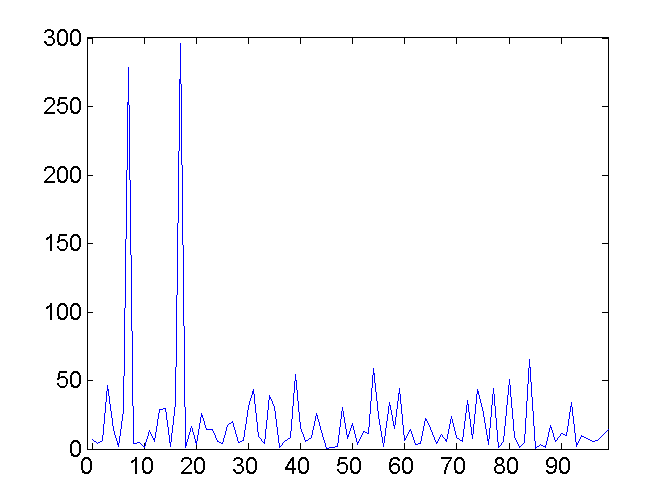
\includegraphics[width=5cm]{img/frequencies.png}
        \caption{Frequencies.}
      \end{minipage}
    \end{figure}
    \end{itemize}
    \end{frame}
  }


  { 
    \setbeamertemplate{footline}{}
    \begin{frame}{What is wavelet transform?}
    \begin{minipage}[b]{0.55\textwidth}
      \begin{itemize}
        \item \textbf{Decomposes a signal into different frequency subbands.}\\
              Applicable to $n$-dimensional signals.
        \item Data transformed to preserve relative distance between objects at different levels of resolution.
        \item Data transformed to preserve relative distance between objects at different levels of resolution.
        \item Allow natural clusters to become more distinguishable.
        \item Used for image compression.
      \end{itemize}
    \end{minipage}\hspace{1cm}
    \begin{minipage}[b]{0.30\textwidth}
      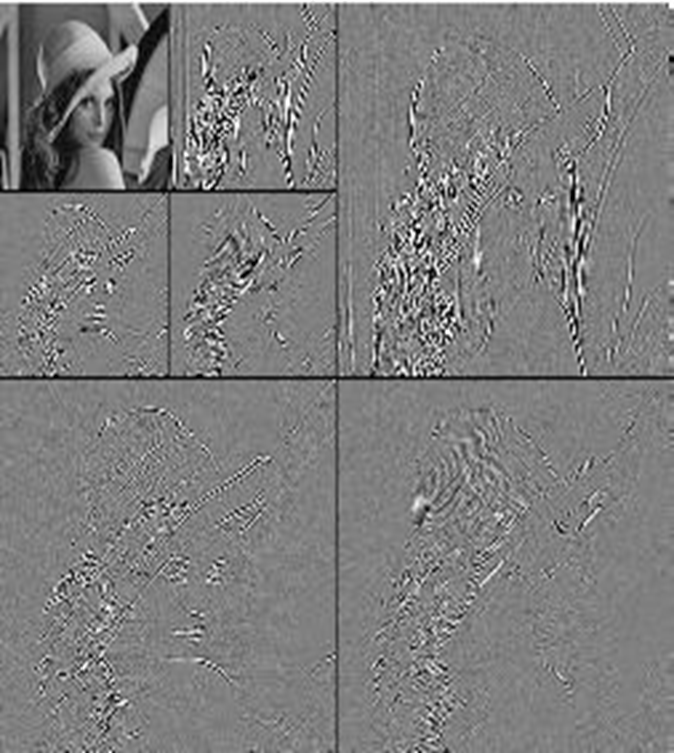
\includegraphics[width=5cm]{img/wavelettransform.png}
    \end{minipage}
    \end{frame}
  }

  { 
    \setbeamertemplate{footline}{}
    \begin{frame}{Wavelet transformation}
    \begin{itemize}
      \item \textbf{Discrete wavelet transform:}\\
            Transforms a vector $X$ into a different vector $X'$ of wavelet coefficients with the same length.
      \item \textbf{Compressed approximation:}\\
            Store only a small fraction of the strongest of the wavelet coefficients.
      \item \textbf{Similar to discrete fourier transform, but better lossy compression, localized in space.}
      \item \textbf{Method:}
      \begin{itemize}
        \item The length of the vector must be an integer power of $2$ (padding with $0$'s if necessary).
        \item Each transform has two functions: smoothing and difference.
        \item Applied to pairs of data, resulting in two sets of data with half the length.
        \item The two functions are applied recursively until reaching the desired length.
      \end{itemize}
    \end{itemize}
    \end{frame}
  }

  {
    \setbeamertemplate{footline}{}
    \begin{frame}{Wavelet decomposition}
    \begin{itemize}
      \item \textbf{Example:}
      \begin{align}
        X &= (2,2,0,2,3,5,4,4), \text{can be transformed to}\\
        X' &= (2.75,-1.25,0.5,0,0,-1,-1,0).
      \end{align}
      \item \textbf{Compression:}\\
            Many small detail coefficients can be replaced by $0$'s, \\
            and only the significant coefficients are retained.
    \end{itemize}
    \vspace{0.2cm}
    \centering
    \begin{tabular}{|c|c|c|}
      \hline
      \text{Resolution} & \text{Averages} & \text{Detail coefficients}\\\hline
      $8$ & $(2,2,0,2,3,5,4,4)$ & - \\\hline
      $4$ & $(2,1,4,4)$ & $(0,-1,-1,0)$ \\\hline
      $2$ & $(1 \frac{1}{2},4)$ & $(\frac{1}{2},0)$ \\\hline
      $1$ & $(2 \frac{3}{4})$ & $(1 \frac{1}{4})$\\\hline
    \end{tabular}
    \end{frame}
  }

  {
    \setbeamertemplate{footline}{}
    \begin{frame}{Why wavelet transform?}
    \begin{itemize}
      \item \textbf{Use hat-shaped filters:}
      \begin{itemize}
        \item Emphasize region where points cluster.
        \item Suppress weaker information in their boundaries.
      \end{itemize}
      \item \textbf{Effective removal of outliers:}
      \begin{itemize}
        \item Insensitive to noise, insensitive to input order.
      \end{itemize}
      \item \textbf{Multi-resolution:}
      \begin{itemize}
        \item Detect arbitrary shaped clusters at different scales.
      \end{itemize}
      \item \textbf{Efficient:} Complexity $\mathcal{O}(N)$.
    \end{itemize}
    \end{frame}
  }

  {
    \setbeamertemplate{footline}{}
    \begin{frame}{Principal component analysis (I)}
    \begin{itemize}
      \item Principal component analysis is a method of summarizing \\
      the properties of a set of multivariate data samples.
      \item It is a \textbf{linear transformation} method that is often used \\ for data analysis or data compression.
      \item Principal component analysis is often also called \textbf{Karhunen-Loeve transformation}.
      \item PCA is equivalent to maximization of the information \\ at the output of a neural network with linear neurons.
    \end{itemize}
    \vspace{0.5cm}
    The goal of the principal component analysis (PCA) is the identification \\
    of $n$ \textbf{normed orthogonal vectors} $\{x_i \in \mathbb{R}^m \; \vert \; i = 1,2, \ldots,n \}$ \\
    within the input space, which \textbf{represent most of the variance} of the data.
    \end{frame}
  }

  {
    \setbeamertemplate{footline}{}
    \begin{frame}{Principal component analysis: the problem (II)}
    \begin{itemize}
    \item Consider sample vectors $u_1, u_2, \ldots, u_n \in \mathbb{R}^m$ centered at zero and a complete orthonormal system $\{x_i \in \mathbb{R}^m \; \vert \; i = 1, 2, \ldots n\}$, such that:
    \begin{align}
      \langle x \rangle &= \int x p(x) d^m x = 0,\\
      \vert\vert u \vert\vert &= 1,\\
      \langle x^{T}u \rangle &= 0,
    \end{align}
    where the Euclidean norm of the vector is given by
    \begin{align}
      \vert\vert u_i \vert\vert = \left(\sum_{i=1}^{m} u_i^2\right)^\frac{1}{2}.
    \end{align}
      \item \textbf{Goal:} find $u^*$ such that $\langle (x^{T}u^*)^2 \rangle$, the variance of the projections of $x$ onto $u^*$ becomes maximal according to the probability distribution $p(x)$.
    \end{itemize}
    \end{frame}
  }

  {
    \setbeamertemplate{footline}{}
    \begin{frame}{Principal component analysis: optimization (III)}
    We seek for the maxima $w^*$ of the following loss function, which represent the variance of the projections of $x$ onto the new basis $u$:
    \begin{align}
      L(w) := \langle (\frac{x^Tw}{\vert\vert w \vert\vert})^2 \rangle = \langle (x^Tu)^2 \rangle = u^T \langle xx^T \rangle = u^T \mathbf{C} u,
    \end{align}
    with
    \begin{align}
      u^* = \frac{w^*}{\vert\vert w^* \vert\vert},
    \end{align}
    because of the fact that
    \begin{align}
      \langle (x^Tw)^2 \rangle = \langle (x^Tw)(x^Tw) \rangle = w^T\langle xx^T \rangle w = w^T \mathbf{C}w,
    \end{align}
    and it holds that
    \begin{align}
      L(w) = \frac{w^T \mathbf{C} w}{\vert\vert w \vert\vert^2}.
    \end{align}
    \end{frame}
  }

  {
    \setbeamertemplate{footline}{}
    \begin{frame}{Principal component analysis: loss function (IV)}
    Extreme values of $L(w)$ correspond to the solution of the following equations:
    \begin{align}
    \nabla_w L(w) &= 0,\\
    \frac{\mathbf{C}w \vert\vert w \vert\vert^2 - (w \mathbf{C} w)w}{\vert\vert w \vert\vert^4} &= 0.
    \end{align}
    This yields the following eigenvalue problem:
    \begin{align}
      \mathbf{C}w = \frac{w\mathbf{C}w}{\vert\vert w \vert\vert^2} \cdot w = L(w) \cdot w = \lambda \cdot w.
    \end{align}
    The above equation yields the eigenvalue problem, which solution is given by
    \begin{align}
    w_i = a \cdot c_i, \; i=1,2,\ldots,n, \; a \in \mathbb{R},
    \end{align}
    i.e. they are parallel to some eigenvector $c_i$ of the correlation matrix $\mathbf{C} = \langle xx^T \rangle$.
    \end{frame}
  }

  {
    \setbeamertemplate{footline}{}
    \begin{frame}{Principal component analysis: principal components (V)}
    \begin{itemize}
      \item For a finite $a \in \mathbb{R}$, there exists a unique maximum with 
      \begin{align}
      w^* = a \cdot c_1.
      \end{align}
      \item The variance of the data becomes maximal for 
      \begin{align}
      u^* = u_1 = \pm c_1.
      \end{align}
      \item This procedure is iterated with the constraint of orthogonality: 
      \begin{align}
      w_k^Tc_l = 0, \; \forall l < k.
      \end{align}
      \item Thus, the eigenvectors are sorted according to descending variance.
    \end{itemize}
    \end{frame}
  }

  {
    \setbeamertemplate{footline}{}
    \begin{frame}{Principal component analysis: principal components (VI)}
    \begin{itemize}
      \item The first principal component corresponds to the eigenvector of the correlation matrix with the largest eigenvalue.
      \item The \textbf{\color{airforceblue}principal components of the data} $x$ are given by the projection of the sample vector $x$ onto the feature vectors $u_i$, such that:
      \begin{align}
        x^Tu_i, \; i = 1, 2, \ldots, m.
      \end{align}
      \item The $k$th component $x^Tu_k$ is along the direction of the eigenvector $u_k$ pointet to the $k$th biggest eigenvalue $\lambda_k$ of the covariance matrix:
      \begin{align}
        \text{Cov}(x) = \langle (x-\mu) (x-\mu)^T \rangle, \; \text{with} \; \mu = \langle x \rangle.
      \end{align}
      \item For centered data, which means if $\mu_k = 0$ then $\forall k$ it holds that the covariance matrix corresponds to the correlation matrix
      \begin{align}
        \mathbf{C} = \langle xx^T \rangle.
      \end{align}
    \end{itemize}
    \end{frame}
  }

  {
    \setbeamertemplate{footline}{}
    \begin{frame}{Principal component analysis: principal components (VII)}
    Consider the variance of the $k$th component along a direction with unit vector $u_k$:
    \begin{align}
      \sigma_{u_k}^2 &= \langle (x^Tu_k)^2 \rangle\\
                     &= \langle u_k^T xx^T u_k \rangle\\
                     &= u_k^T \mathbf{C} u_k\\
                     &= \sum_{\alpha = 1}^{l}\lambda_{\alpha}u_{k\alpha}^2.
    \end{align}
    $u_{k\alpha}$ is the component of $u_k$ along the eigenvector $c_\alpha$ of the matrix $\mathbf{C}$ to the eigenvalue $\lambda_\alpha$.

    Consider, that
    \begin{align}
      \sigma_{u_k}^{2} = \lambda_k, \quad \text{if} \; u_k \vert \vert c_k.
    \end{align}
    The eigenvalues of the covariance matrix correspond to the variance of the feature vector along the principal component $u_i$.
    \end{frame}
  }

  { 
    \setbeamertemplate{footline}{}
    \begin{frame}{}

    \end{frame}
  }

  { 
    \setbeamertemplate{footline}{}
    \begin{frame}{Types of sampling}
        \begin{itemize}
            \item \textbf{Simple random sampling.}
            \begin{itemize}
              \item There is an equal probability of selecting any particular item.
            \end{itemize}
            \item \textbf{Sampling without repetition.}
            \begin{itemize}
              \item Once an object is selected, it is removed from the population.
            \end{itemize}
            \item \textbf{Sampling with repetition.}
            \begin{itemize}
              \item A selected object is not removed from the population.
            \end{itemize}
            \item \textbf{Stratified sampling:}
            \begin{itemize}
              \item Partition the data set and draw samples from each partition: Proportionally, i.e. approximately the same percentage of the data.
              \item Used in conjunction with skewed data.
            \end{itemize}
        \end{itemize}
    \end{frame}
  }


  { 
    \setbeamertemplate{footline}{}
    \begin{frame}{Data-cube aggregation}
        \begin{itemize}
            \item \textbf{The lowest level of a data cube (base cuboid).}
            \begin{itemize}
              \item The aggregated data for an \textbf{individual entity of interest}.
              \item E.g. a customer in a phone-calling data warehouse.
              \item Number of calls per hour, day, or week.
            \end{itemize}
            \item \textbf{Multiple levels of aggregation in data cubes.}
            \begin{itemize}
              \item Further reduce the size of data to deal with.
            \end{itemize}
            \item \textbf{Reference appropriate levels.}
            \begin{itemize}
              \item Use the smallest representation which is enough to solve the task.
            \end{itemize}
            \item \textbf{Queries regarding aggregated information should be answered using the data cube, if possible.}
        \end{itemize}
    \end{frame}
  }

  { 
    \setbeamertemplate{footline}{}
    \begin{frame}{Data reduction (III): data compression}
        \begin{itemize}
            \item \textbf{String compression.}
            \begin{itemize}
              \item There are extensive theories and well-tuned algorithms.
              \item Typically lossless, but only limited manipulation is possible without expansion.
            \end{itemize}
            \item \textbf{Audio/video compression.}
            \begin{itemize}
              \item Typically lossy compression, with progressive refinement.
              \item Sometimes small fragments of signal can be reconstructed without reconstructing the whole.
            \end{itemize}
            \item \textbf{Time sequence is not audio.}
            \begin{itemize}
              \item Typically short and varies slowly with time.
            \end{itemize}
            \item \textbf{Dimensionality and numerosity reduction may also be considered as forms of data compression.}
        \end{itemize}
    \end{frame}
  }

  { 
    \setbeamertemplate{footline}{}
    \begin{frame}{Chapter IV: Preprocessing}
        \begin{itemize}
            \item Data preprocessing: an overview.
            \begin{itemize}
              \item Data quality.
              \item Major tasks in data preprocessing.
            \end{itemize}
            \item Data cleaning.
            \item Data integration.
            \item Data reduction.
            \item \textbf{Data transformation and data discretization.}
            \item Summary.
        \end{itemize}
    \end{frame}
  }

 {
    \setbeamertemplate{footline}{}
    \begin{frame}{Data transformations}
    \begin{itemize}
      \item Functions applied to a finite set of samples.
      \item \textbf{Methods:}
      \begin{itemize}
        \item Smoothing: Remove noise from data.
        \item Attribute/feature construction: New attributes constructed from the given ones.
        \item Aggregation: Summarization, data-cube construction.
        \item Normalization: Scaled to fall within a smaller, specified range.
        \begin{itemize}
          \item Min-max normalization
          \item Z-score normalization.
          \item Normalization by decimal scaling.
        \end{itemize}
        \item Discretization: concept-hierarchy climbing.
      \end{itemize}
    \end{itemize}
    \end{frame}
  }

  {
    \setbeamertemplate{footline}{}
    \begin{frame}{Normalization}
      \begin{itemize}
        \item \textbf{Min-max normalization (to some interval $[\text{min},\text{max}]$:}
        \begin{align}
          a_{\text{new}} = \frac{a - \text{min}_A}{\text{max}_A-\min_{A}} (\max - \min) + \min.
        \end{align}
        Example: let income range from $\$12.000$ to $\$98.000$ normalized to $[0,1]$.\\
        Then $\$73.600$ is mapped to $\frac{73.600-12.000}{98.000-12.000} (1-0) + 0 = 0.716$.
        \item \textbf{Z-score normalization:}
        \begin{align}
          x_{\text{new}} := z = \frac{a-\mu_{A}}{\sigma_A}, \; \text{with $\mu$ being the mean and $\sigma$ the standard deviation.}
        \end{align}
        Example: let $\mu = 54.000$ and $\sigma = 16.000$. Then $\frac{73.000-54.000}{16.000} = 1.225$.
        \item \textbf{Normalization by decimal scaling:}
        \begin{align}
        a_{\text{new}} = \frac{a}{10^k}, \; \text{where $k$ is the smallest integer such that} \; \max(\vert a_{\text{new}} \vert) < 1.
        \end{align}
      \end{itemize}
    \end{frame}
  }

  {
    \setbeamertemplate{footline}{}
    \begin{frame}{Discretization}
    \begin{itemize}
      \item \textbf{Three types of attributes:}
      \begin{itemize}
        \item Nominal -- values from an unordered set, e.g. color, profession.
        \item Ordinal -- values from an ordered set, e.g. military or academic rank.
        \item Numerical -- numbers, e.g. integer or real numbers.
      \end{itemize}
      \item \textbf{Divide the value range of a continuous attribute into intervals:}
      \begin{itemize}
        \item \textbf{Interval labels} can then be used to replace actual data values.
        \item Reduce data size by discretization.
        \item Supervised vs. unsupervised.
        \item Split (top-down) vs. merge (bottom-up).
        \item Discretization can be performed recursively on an attribute.
        \item Prepare for further analysis, e.g. classification.
      \end{itemize}
    \end{itemize}
    \end{frame}
  }

  {
    \setbeamertemplate{footline}{}
    \begin{frame}{Data-discretization Methods}
    \begin{itemize}
      \item \textbf{Typical methods:}
      \begin{itemize}
        \item All the methods can be applied recursively.
        \item \textbf{Binning:}
              \begin{itemize}
                \item Unsupervised, top-down split.
              \end{itemize}
        \item \textbf{Histogram analysis:}
              \begin{itemize}
                \item Unsupervised, top-down split.
              \end{itemize}
        \item \textbf{Clustering analysis:}
              \begin{itemize}
                \item Unsupervised, top-down split or bottom-up merge.
              \end{itemize}
        \item \textbf{Decision-tree analysis:}
              \begin{itemize}
                \item Supervised, top-down split.
              \end{itemize}
        \item \textbf{Correlation (e.g., $\chi^2$) analysis:}
              \begin{itemize}
                \item Unsupervised, bottom-up merge.
              \end{itemize}
      \end{itemize}
    \end{itemize}
    \end{frame}
  }

  {
    \setbeamertemplate{footline}{}
    \begin{frame}{Simple discretization: binning}
    \begin{itemize}
      \item \textbf{Equal-width (distance) partitioning:}
      \begin{itemize}
        \item Divides the range into $N$ intervals of equal size: uniform grid.
        \item If $A$ and $B$ are the lowest and highest values of the attribute, the width of intervals will be: $W = \frac{(B - A)}{N}$.
        \item The most straightforward, but outliers may dominate presentation.
        \item Skewed data is not handled well.
      \end{itemize}
      \item \textbf{Equal-depth (frequency) partitioning:}
      \begin{itemize}
        \item Divides the range into $N$ intervals, each containing approximately same number of samples.
        \item Good data scaling.
        \item Managing categorical attributes can be tricky.
      \end{itemize}
    \end{itemize}
    \end{frame}
  }

  {
    \setbeamertemplate{footline}{}
    \begin{frame}{Binning methods for data smoothing}
    \begin{itemize}
      \item \textbf{Sorted data for price (in dollars):} \\
            $4, 8, 9, 15, 21, 21, 24, 25, 26, 28, 29, 34$.
      \item \textbf{Partition into equal-frequency (equal-depth) bins:}\\
            Bin $1$: $4, 8, 9, 15$,\\
            Bin $2$: $21, 21, 24, 25$,\\
            Bin $3$: $26, 28, 29, 34$.
      \item \textbf{Smoothing by bin means:}\\
            Bin $1$: $9, 9, 9, 9$,\\
            Bin $2$: $23, 23, 23, 23$,\\
            Bin $3$: $29, 29, 29, 29$.\\
      \item \textbf{Smoothing by bin boundaries:}\\
            Bin $1$: $4, 4, 4, 15$,\\
            Bin $2$: $21, 21, 25, 25$,\\
            Bin $3$: $26, 26, 26, 34$.\\
    \end{itemize}
    \end{frame}
  }

  { 
    \setbeamertemplate{footline}{}
    \begin{frame}{Discretization without using class labels (binning vs. clustering)}
    \begin{figure}[H]
        \centering
        \begin{minipage}{0.32\textwidth}
            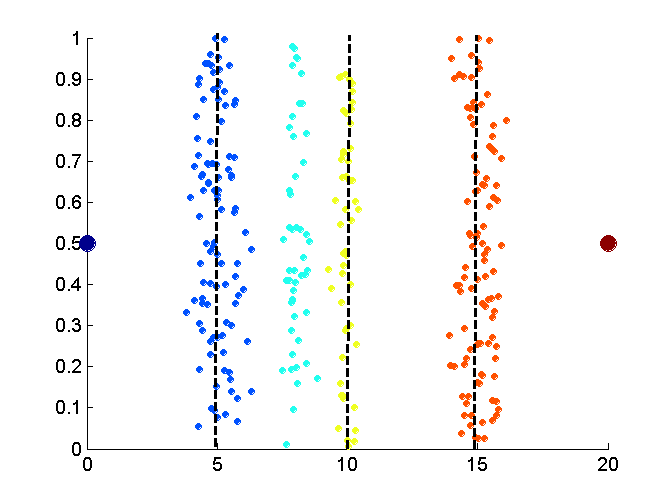
\includegraphics[width=5cm]{img/binningvsclustering2.png}
            \caption{a) Equal interval width (binning).}
        \end{minipage}
        \begin{minipage}{0.32\textwidth}
            \centering
            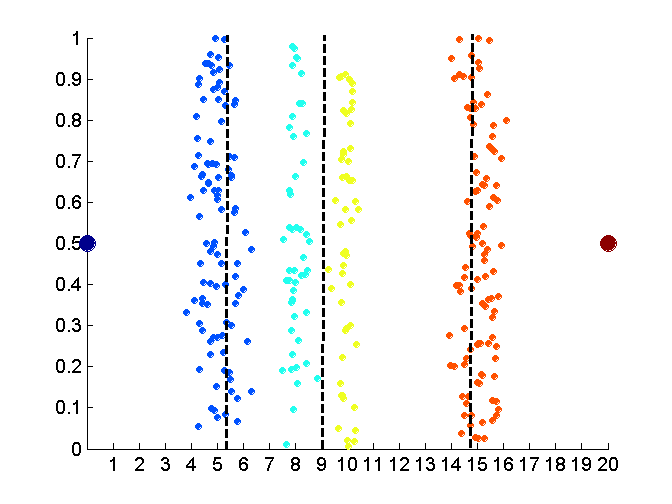
\includegraphics[width=5cm]{img/binningvsclustering3.png}
            \caption{b) Equal frequency (binning).}
        \end{minipage}
        \begin{minipage}{0.32\textwidth}
            \centering
            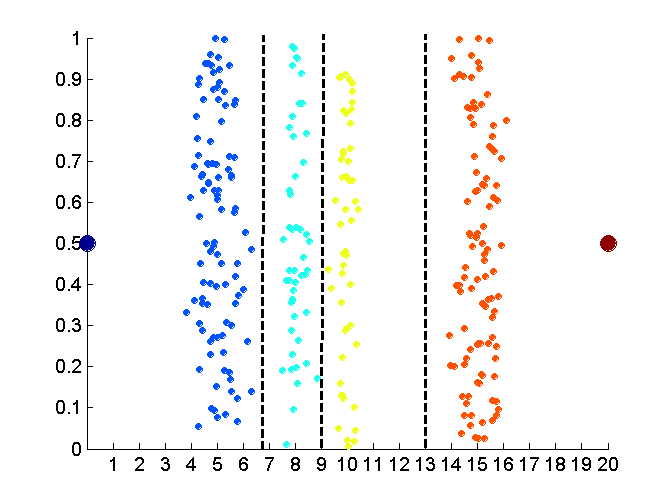
\includegraphics[width=5cm]{img/binningvsclustering4.png}
            \caption{c) K-means clustering.}
        \end{minipage}\hfill
    \end{figure} 
    \end{frame}
  }

  { 
    \setbeamertemplate{footline}{}
    \begin{frame}{Discretization by classification \& correlation analysis}
        \begin{itemize}
            \item \textbf{Classification:}
            \begin{itemize}
              \item E.g. decision-tree analysis.
              \item Supervised: Class labels given for training set e.g. cancerous vs. benign.
              \item Using \textbf{entropy} to determine split point (discretization point).
              \item Top-down, recursive split.
              \item Details will be covered in Chapter 6.
            \end{itemize}
            \item \textbf{Correlation analysis:}
            \begin{itemize}
              \item E.g. $\chi^2$-merge: $\chi^2$-based discretization.
              \item Supervised: use class information.
              \item Bottom-up merge: find the best neighboring intervals (those having similar distributions of classes, i.e., low $\chi^2$ values) to merge.
              \item Merge performed recursively, until a predefined stopping condition.
            \end{itemize}
        \end{itemize}
    \end{frame}
  }


  { 
    \setbeamertemplate{footline}{}
    \begin{frame}{Concept-hierarchy generation}
        \begin{itemize}
            \item \textbf{Concept hierarchy:}
            \begin{itemize}
              \item Organizes concepts (i.e. attribute values) hierarchically.
              \item Usually associated with each dimension in a data warehouse.
              \item Facilitates \textbf{drilling and rolling} in data warehouses to view data at multiple granularity.
            \end{itemize}
            \item \textbf{Concept-hierarchy formation:}
            \begin{itemize}
              \item Recursively reduce the data by collecting and replacing \textbf{low-level concepts} (such as numerical values for age) by \textbf{higher-level concepts} (such as youth, adult, or senior).
              \item Can be explicitly specified by domain experts and/or data-warehouse designers.
              \item Can be automatically formed for both numerical and nominal data.
              \item For numerical data, use discretization methods shown.
            \end{itemize}
        \end{itemize}
    \end{frame}
  }

  { 
    \setbeamertemplate{footline}{}
    \begin{frame}{Concept-hierarchy generation for nominal data}
        \begin{itemize}
            \item \textbf{Specification of a partial/total ordering of attributes explicitly at the schema level by users or experts.}
            \begin{itemize}
              \item $\#(\text{streets}) < \#(\text{city}) < \#(\text{state}) < \#(\text{country})$.
            \end{itemize}
            \item \textbf{Specification of a hierarchy for a set of values by explicit data grouping.}
            \begin{itemize}
              \item $\#(\{"Urbana", "Champaign", "Chicago"\}) < \#(\text{Illinois})$.
            \end{itemize}
            \item \textbf{Specification of only a partial set of attributes.}
            \begin{itemize}
              \item Only $\#(\text{street}) < \#(\text{city})$, not others.
            \end{itemize}
            \item \textbf{Automatic generation of hierarchies (or attribute levels) by the analysis of the number of distinct values.}
            \begin{itemize}
              \item E.g. for a set of attributes: $\{\text{street}, \text{city}, \text{state}, \text{country}\}$.
              \item See on the next slides.
            \end{itemize}
        \end{itemize}
    \end{frame}
  }

  { 
    \setbeamertemplate{footline}{}
    \begin{frame}{Automatic concept-hierarchy generation}
        \begin{itemize}
            \item \textbf{Some hierarchies can be automatically generated based on the analysis of the number of distinct values per attribute.}
            \begin{itemize}
              \item The attribute with the most distinct values is placed at the lowest level of the hierarchy.
              \item Exceptions, e.g. weekday, month, quarter, year.
            \end{itemize}
            \item Example: 
            \begin{align}
            \#(\text{streets} &= 674.339 > \#(\text{city}) =  3567,\\
            \#(\text{city}) &=  3567 > \#(\text{province or state}) =  356,\\
            \#(\text{province or state}) &=  356 > \#(\text{country}) = 15.
            \end{align}
        \end{itemize}
    \end{frame}
  }

  { 
    \setbeamertemplate{footline}{}
    \begin{frame}{Chapter IV: Preprocessing}
        \begin{itemize}
            \item Data preprocessing: an overview.
            \begin{itemize}
              \item Data quality.
              \item Major tasks in data preprocessing.
            \end{itemize}
            \item Data cleaning.
            \item Data integration.
            \item Data reduction.
            \item Data transformation and data discretization.
            \item \textbf{Summary.}
        \end{itemize}
    \end{frame}
  }

  {
    \setbeamertemplate{footline}{}
    \begin{frame}{Summary}
      \begin{itemize}
        \item \textbf{Data quality:} Accuracy, completeness, consistency, timeliness, believability, interpretability.
        \item \textbf{Data cleaning:} E.g. missing/noisy values, outliers.
        \item \textbf{Data integraiom from multiple sources:}
        \begin{itemize}
          \item Entity identification problem.
          \item Remove redundancies.
          \item Detect inconsistencies.
        \end{itemize}
        \item \textbf{Data reduction:}
        \begin{itemize}
          \item Dimensionality reduction.
          \item Numerosity reduction.
          \item Data compression.
        \end{itemize}
        \item \textbf{Data transformation and data discretization:}
        \begin{itemize}
          \item Normalization.
          \item Concept-hierarchy generation.
        \end{itemize}
      \end{itemize}
    \end{frame}
  }


  {
    \setbeamertemplate{footline}{}
    \begin{frame}{References (I)}
      \begin{itemize}
        \item D. P. Ballou and G. K. Tayi: Enhancing data quality in data warehouse environments. Comm. of ACM, 42:73-78, 1999.
        \item A. Bruce, D. Donoho, and H.-Y. Gao: Wavelet analysis. IEEE Spectrum, Oct. 1996.
        \item {\color{airforceblue}T. Dasu and T. Johnson:  Exploratory Data Mining and Data Cleaning. John Wiley, 2003.}
        \item J. Devore and R. Peck: Statistics: The Exploration and Analysis of Data. Duxbury Press, 1997.
        \item H. Galhardas, D. Florescu, D. Shasha, E. Simon, and C.-A. Saita: Declarative data cleaning: Language, model, and algorithms. VLDB'01.
        \item M. Hua and J. Pei: Cleaning disguised missing data: A heuristic approach. KDD'07.
        \item {\color{airforceblue}H. V. Jagadish et al.: Special Issue on Data Reduction Techniques.  Bulletin of the Technical Committee on Data Engineering, 20(4), Dec. 1997.}
      \end{itemize}
    \end{frame}
  }


  {
    \setbeamertemplate{footline}{}
    \begin{frame}{References (2)}
      \begin{itemize}
        \item H. Liu and H. Motoda (eds.): Feature Extraction, Construction, and Selection: A Data Mining Perspective. Kluwer Academic, 1998.
        \item J. E. Olson. Data Quality: The Accuracy Dimension. Morgan Kaufmann, 2003.
        \item D. Pyle: Data Preparation for Data Mining. Morgan Kaufmann, 1999.
        \item {\color{airforceblue}V. Raman and J. Hellerstein: Potter's Wheel: An Interactive Framework for Data Cleaning and Transformation, VLDB'01.}
        \item T. Redman: Data Quality: The Field Guide. Digital Press (Elsevier), 2001.
        \item R. Wang, V. Storey, and C. Firth: A framework for analysis of data quality research. IEEE Trans. Knowledge and Data Engineering, 7:623-640, 1995.
      \end{itemize}
    \end{frame}
  }

  { % Questions?
    \setbeamertemplate{footline}{}
    \begin{frame}[c]
      \begin{center}
        Thank you for your attention.\\
        {\bf Any questions about the forth chapter?}\\[0.5cm]
        Ask them now, or again, drop me a line: \\ 
        \faSendO \ \texttt{luciano.melodia@fau.de}.
      \end{center}
    \end{frame}
  }
\end{document}

